% =====================================================================
%  Figure blocks and captions for "Catalytic Ladder Propagation".
%
%  Every number quoted in these captions is read from the JSON written by
%  validation/exp_{a,b,c,d}.py and is reproduced by make_figures.py from
%  the same values.  Where a panel reports a quantity the suite marks as
%  illustrative rather than measured, the caption says so.
% =====================================================================

% ---------------------------------------------------------------------
\begin{figure*}[!htbp]
    \centering
    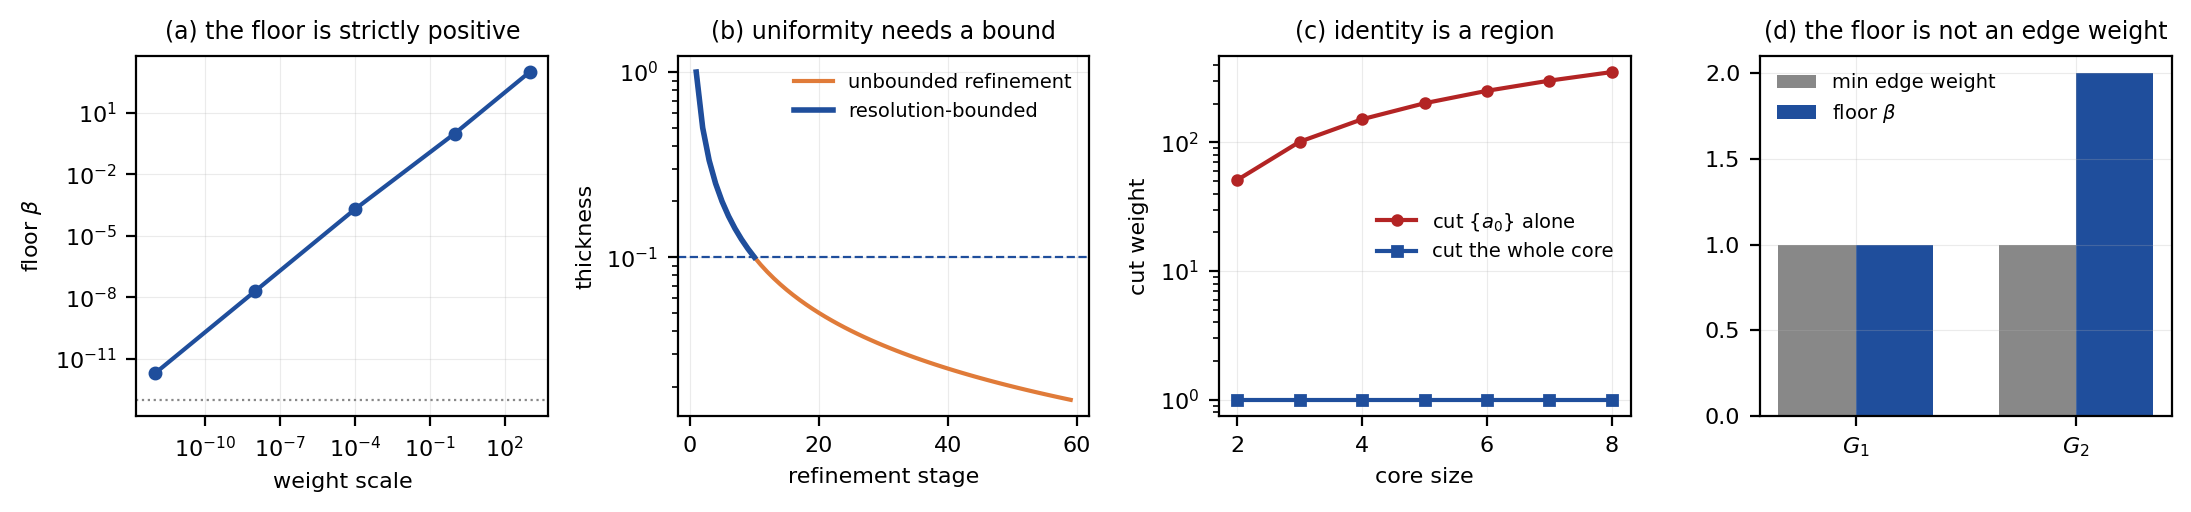
\includegraphics[width=\textwidth]{figures/fig1_substrate.png}
    \caption{\textbf{The floor is computed, the uniformity hypothesis does
    real work, and identity is a region rather than a point.}
    \textbf{(A)}~Contact floor $\beta$ computed---not assumed---over instances
    spanning twelve orders of magnitude of weight scale, including an
    adversarial case whose smallest edge weight is $10^{-12}$. Every instance
    returns a strictly positive floor. The adversarial instance is the
    informative one: its floor is $1+10^{-12}$ and \emph{not} $10^{-12}$,
    because that light edge lies inside every cut that would use it, and a
    cheap edge inside an expensive cut does not make the cut cheap. Positivity
    follows from finiteness and strict positivity of the weights, not from
    their scale.
    \textbf{(B)}~The failure branch, drawn so the hypothesis is visible rather
    than tacit. A system permitted to refine without limit generates
    thicknesses $1/n$ (orange): each is strictly positive while the infimum is
    zero, and every $\varepsilon$ in a ladder down to $2.5\times10^{-3}$ is
    eventually cleared. Truncating the same sequence to a resolution-bounded
    system (blue, first ten stages) restores a positive floor at $0.1$
    (dashed). Theorem~\ref{thm:floor} is unconditional; the uniform statement
    of Theorem~\ref{thm:uniform} is not, and every result downstream inherits
    the condition.
    \textbf{(C)}~Identity is a region and not a point
    (Proposition~\ref{prop:region}). For a vertex buried in a clique of
    internal weight $W=50$, severing it alone from the core costs $W(n-1)+1$
    and grows with core size (red), while severing the whole core from its
    surroundings costs $1$ regardless (blue). Exhaustive enumeration confirms
    every minimiser contains all four core vertices. Read chemically: the
    identity of a residue in a packed core---what it is separated from, and at
    what cost---is a property of the core, so any scheme assigning identity
    residue-by-residue is assigning something other than identity.
    \textbf{(D)}~The floor is not an edge weight, and the difference is what
    Theorem~\ref{thm:separation} turns on. Two contact graphs with
    \emph{identical} minimum edge weight $1.0$ (grey) have floors $1$ and $2$
    (blue). A query over stored weights sees the grey bars; the accountability
    verdict depends on the blue ones.}
    \label{fig:substrate}
\end{figure*}

% ---------------------------------------------------------------------
\begin{figure*}[!htbp]
    \centering
    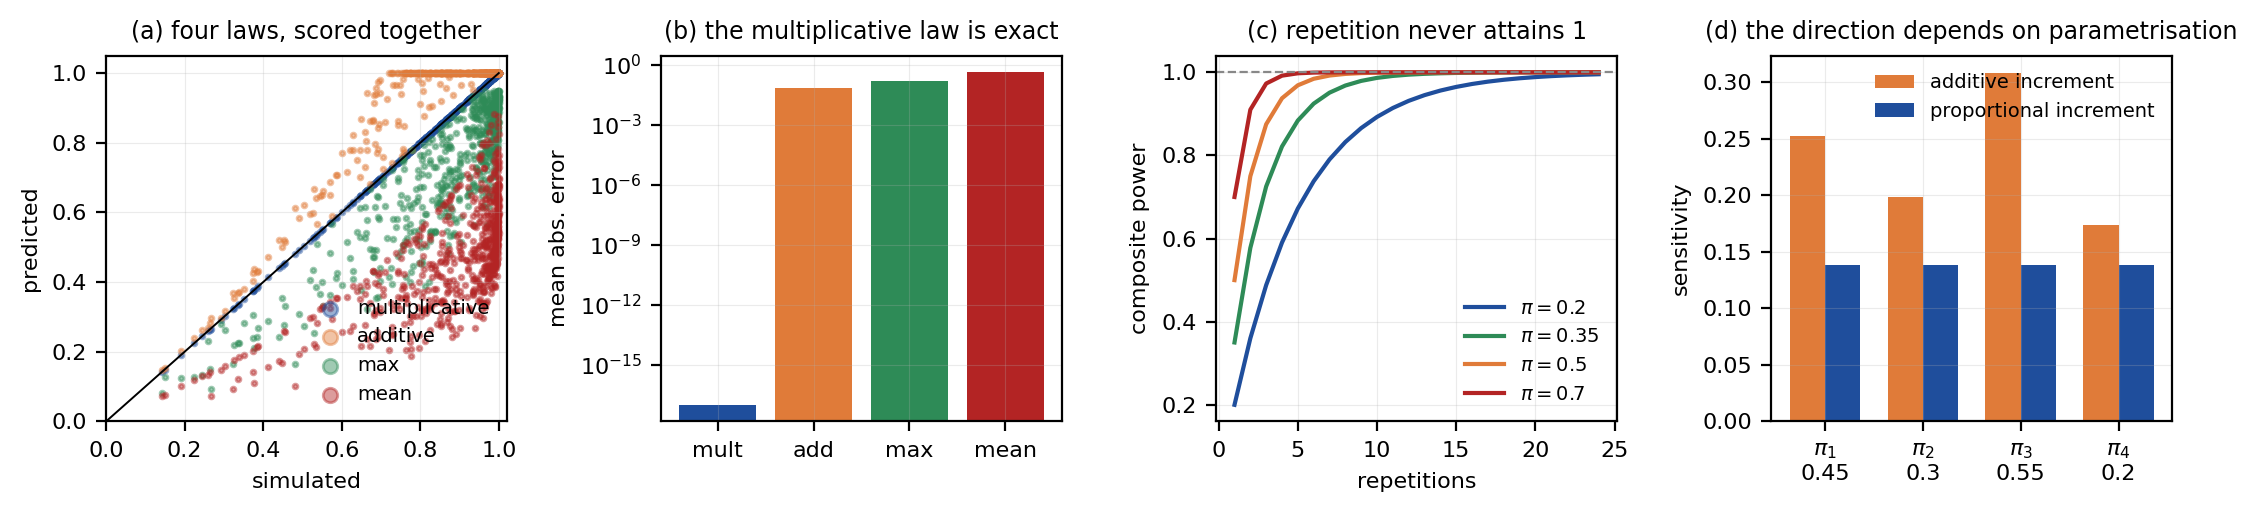
\includegraphics[width=\textwidth]{figures/fig2_ladder.png}
    \caption{\textbf{Composition is multiplicative, repetition saturates, and
    the counter-intuitive direction of control is a property of the
    parametrisation.}
    \textbf{(A)}~Predicted against simulated composite power for four candidate
    composition laws on randomly generated ladders, scored against a
    rung-by-rung simulation of the residual gap. The multiplicative law lies on
    the identity; the additive law saturates and overshoots, the maximum law
    systematically underestimates, and the mean law fails badly. The comparison
    is the test: scoring only the favoured law would not have distinguished it
    from the others.
    \textbf{(B)}~Mean absolute error by law over $4000$ ladders, on a
    logarithmic axis. The multiplicative law is exact to machine precision
    ($0.0$); the alternatives err by $5.45\times10^{-2}$,
    $1.49\times10^{-1}$ and $4.31\times10^{-1}$. The gap is not a matter of fit
    quality but of which law is true.
    \textbf{(C)}~Composite power under repetition of a single rung, for four
    rung powers. Each curve rises strictly, tends to unity (dashed), and
    reaches it at no finite $n$; the $n$-th repetition contributes
    $\pi(1-\pi)^{n-1}$. Copies of what already works have geometrically
    diminishing returns, so a ladder of near-duplicate rungs cannot attain a
    demanding target however long it is made.
    \textbf{(D)}~The correction of Remark~\ref{rem:sens-honest}, and the reason
    this panel exists. Under an \emph{additive} increment applied equally at
    every rung (orange) the sensitivity $\prod_{i\neq j}(1-\pi_i)$ varies
    across rungs and is maximised at the \emph{strongest}, $\pi_3=0.55$---the
    counter-intuitive direction, reproduced here in $5000/5000$ ladders. Under
    a \emph{proportional} increment, raising a rung by a fixed fraction of its
    own headroom, the factors cancel and the sensitivity is identical at every
    rung (blue): measured spread $1.11\times10^{-16}$, machine zero, in
    $5000/5000$ ladders. Which parametrisation applies is an empirical question
    about how improvements are purchased, and a check comparing the analytic
    derivative against a numerical one cannot detect the difference, because
    both quantities are the same additive derivative.}
    \label{fig:ladder}
\end{figure*}

% ---------------------------------------------------------------------
\begin{figure*}[!htbp]
    \centering
    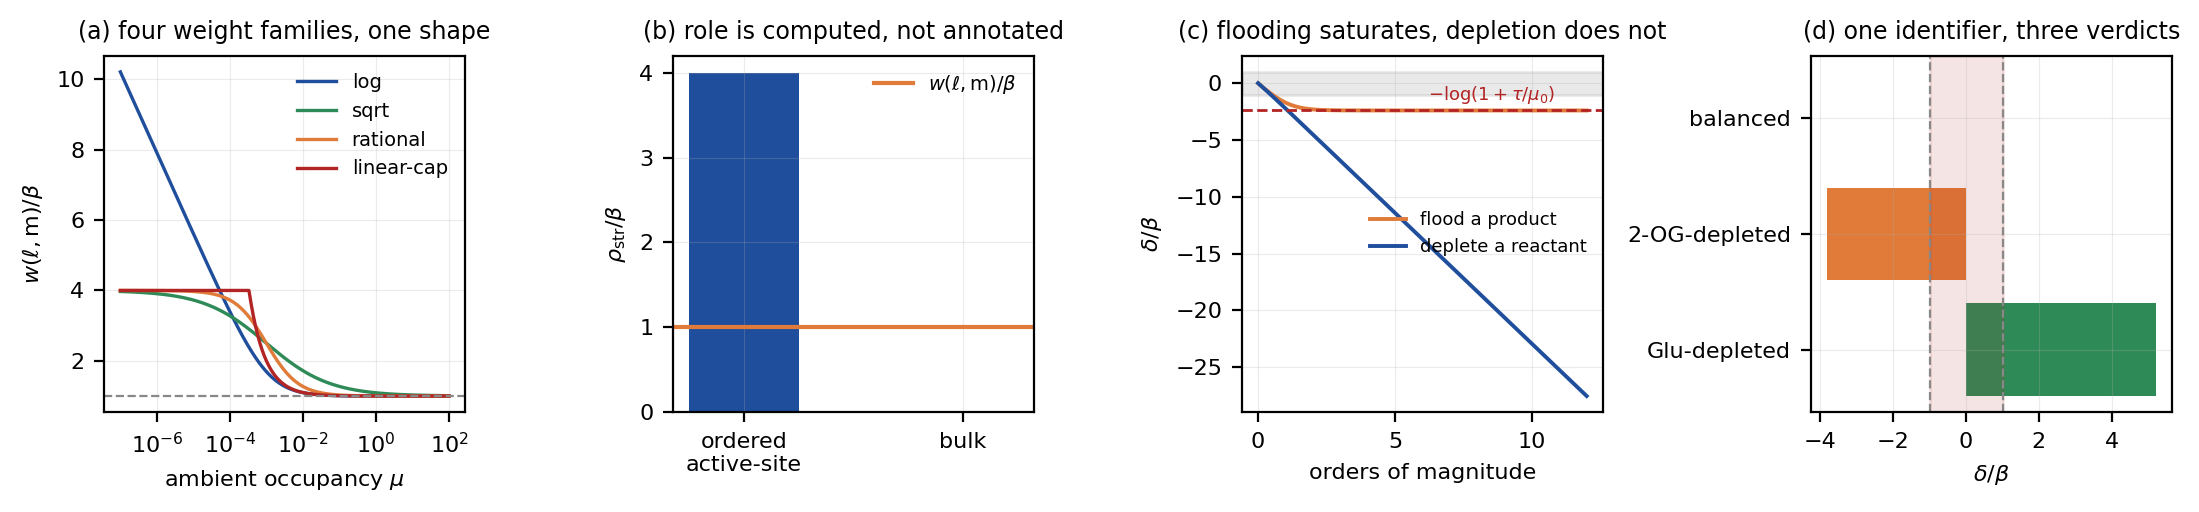
\includegraphics[width=\textwidth]{figures/fig3_medium.png}
    \caption{\textbf{The medium decides solvent role and reaction direction,
    and one asymmetry in it was found by a test written to be capable of
    failing.}
    \textbf{(A)}~Four weight families satisfying the two properties the
    theorems actually use---strictly decreasing in ambient occupancy and
    bounded below by the floor (dashed). Logarithmic, square-root, rational and
    a non-smooth linear cap are otherwise unrelated. Every structural result in
    Section~\ref{sec:medium} is re-verified under all four, so no theorem
    depends on the constitutive choice of Equation~\eqref{eq:mediumweight};
    only the numerical values do, and those are illustrative.
    \textbf{(B)}~Solvent role is computed, not annotated
    (Theorem~\ref{thm:role}). Two waters of identical chemical identity receive
    opposite roles: the ordered active-site water holds
    $\rho_{\mathrm{str}}=4\beta$ against the system and is \textsf{structural};
    the bulk water holds none and is \textsf{bulk}. The orange line is the
    competing boundary $w(\ell,\mathsf{m})=1.000\,\beta$, computed at ambient
    water. This is the distinction a five-class leaf algebra with one
    \textsf{solvent} class cannot draw, and no curator supplies it.
    \textbf{(C)}~The saturation asymmetry of
    Proposition~\ref{prop:saturation}, which we did not anticipate. Flooding a
    product (orange) approaches the ceiling
    $-\log(1+\tau/\mu_0)=-2.397895\,\beta$ (red dashed) and stops: thirty
    orders of magnitude of further flooding move it no further, and the
    measured limit agrees with the predicted one to six decimal places.
    Depleting a reactant (blue) descends without bound, reaching
    $-22.93\,\beta$ over the same range. Read chemically, product inhibition
    cannot reverse a reaction and only substrate depletion can. The grey band
    is the refusal region $\lvert\delta\rvert\leq\beta$. This result exists
    because an earlier one-sided sweep never reached case~(b) of
    Theorem~\ref{thm:trichotomy} and looked like a refutation; the theorem was
    not at fault, the sweep was.
    \textbf{(D)}~One reaction identifier, three verdicts
    (Corollary~\ref{cor:oneidentifier}). The same chain, with the same
    participants and the same identifier, is forward at $\delta=+5.204\,\beta$
    in a glutamate-depleted cytosol, reverse at $-3.818\,\beta$ in a
    2-oxoglutarate-depleted one, and undirected at exactly $0$ in a balanced
    medium. The third is a negative control: without a medium that
    \emph{refuses} to orient, the trichotomy would be a dichotomy with a
    decorative third branch.}
    \label{fig:medium}
\end{figure*}

% ---------------------------------------------------------------------
\begin{figure*}[!htbp]
    \centering
    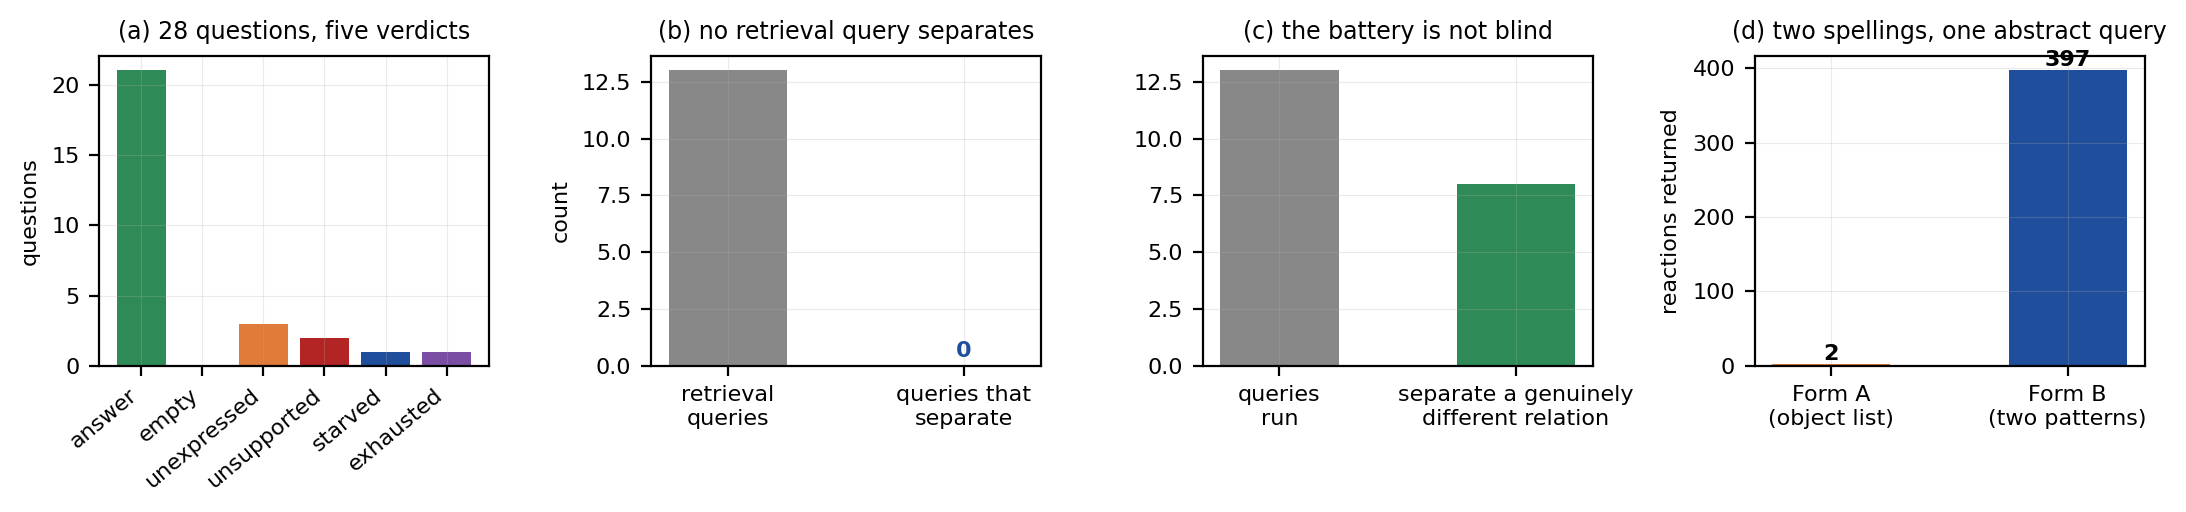
\includegraphics[width=\textwidth]{figures/fig4_verdicts.png}
    \caption{\textbf{Twenty-eight questions, five verdicts, and the
    expressibility separation executed rather than argued.}
    \textbf{(A)}~The twenty-eight questions by verdict: $21$ answered, $3$
    \textsf{unexpressed}, $2$ \textsf{unsupported}, $1$ \textsf{starved} and
    $1$ \textsf{exhausted}. Twelve of the questions were supplied by
    practitioners without reference to this framework and sixteen were added to
    reach outcomes the twelve do not. Every refusal carries a named blocker and
    a statement of what would unblock it. A system that answered all
    twenty-eight would have an empty defined class: it would not classify, it
    would merely accept.
    \textbf{(B)}~The separation of Theorem~\ref{thm:separation}, measured.
    Thirteen retrieval query forms---triple enumeration, counts, grouped
    degree, neighbourhoods, two \textsf{ASK} forms over property paths,
    transitive closure, two-hop joins, \textsf{OPTIONAL} with \textsf{FILTER},
    and a nested aggregate---were run against two contact graphs recording
    identical triples, on two independently developed SPARQL engines
    (\texttt{rdflib} 7.6.0 and \texttt{pyoxigraph} 0.5.9). The two engines
    agreed on every query, and \emph{none} of the thirteen separated the two
    systems, while their accountability verdicts differ: $\sigma(v_0,x)=2$ in
    both, with floors $1$ and $2$.
    \textbf{(C)}~The negative control, which is the load-bearing panel. The
    same battery run against a third graph with a genuinely different contact
    relation separates it on $8$ of the $13$ queries. Without this, the null
    result in~(B) would be consistent with a blind battery rather than with a
    property of the two systems.
    \textbf{(D)}~The live divergence of Section~\ref{sec:res-d}. Two spellings
    that SPARQL~1.1 defines as one abstract query---an object list against two
    triple patterns---return $2$ and $397$ against the same public endpoint on
    the same date, while both spellings agree with each other and with hand
    computation on a miniature of the same data shape run on both local
    engines. The divergence is established; its cause is not, and we declined
    to diagnose a third party's service.}
    \label{fig:verdicts}
\end{figure*}
